\section{Client-Server Architecture}

One of the first technical design decisions to be discussed was that of the client-server architecture and how the different clients would keep synchronised with each other. This was a very important decision to make as a poor networking set up can severely impact the playability of the game. For example, Patrick Wyatt talks about how the first ever multiplayer game of \emph{Warcraft} experienced a serious game-state synchronisation problem; both computers involved ended up ``showing entirely different battles that, while they started identically, diverged into two entirely different universes''.\cite{wyatt2012warcraft} Three separate strategies for solving this problem were discussed: lockstep, simple server-client, and server-client with simulation.

Lockstep is a peer-to-peer strategy in which each computer has a full model of the game state. Whenever a client's game state changes they must send this update to all of the other clients to apply to their copies of the game state too. There is no centralised server in this networking model, so disconnection of a single client does not cause the game to stop. It also allows users to play games on networks with high latency without actually experiencing any perceived lag. This is because clients apply delayed packets as they arrive. The robustness afforded by this technique is highly desirable for games with long playing times, such as Sid Meier's Civilisation.\sidenote{Sid Meier's Civilization is a turn-based strategy game, for more information see \url{civilization.com}.}

However, maintaining synchronisation when using a peer-to-peer protocol like this can be very challenging. The clients have to be able to collectively handle messages arriving in different orders for each individual. If this happens the game can start to desynchronise and the games will ultimately diverge. For example, Figure~\ref{fig:serverClientDesync} shows how two clients can easily diverge. Each pair of grids in the diagram represents the state of the game for each client, with client one on the left and client two on the right, at the given time step. Client one sees the blue character successfully hit the red character, but client two sees the red character step out of the way and the blue player's shot misses.

\begin{marginfigure}
	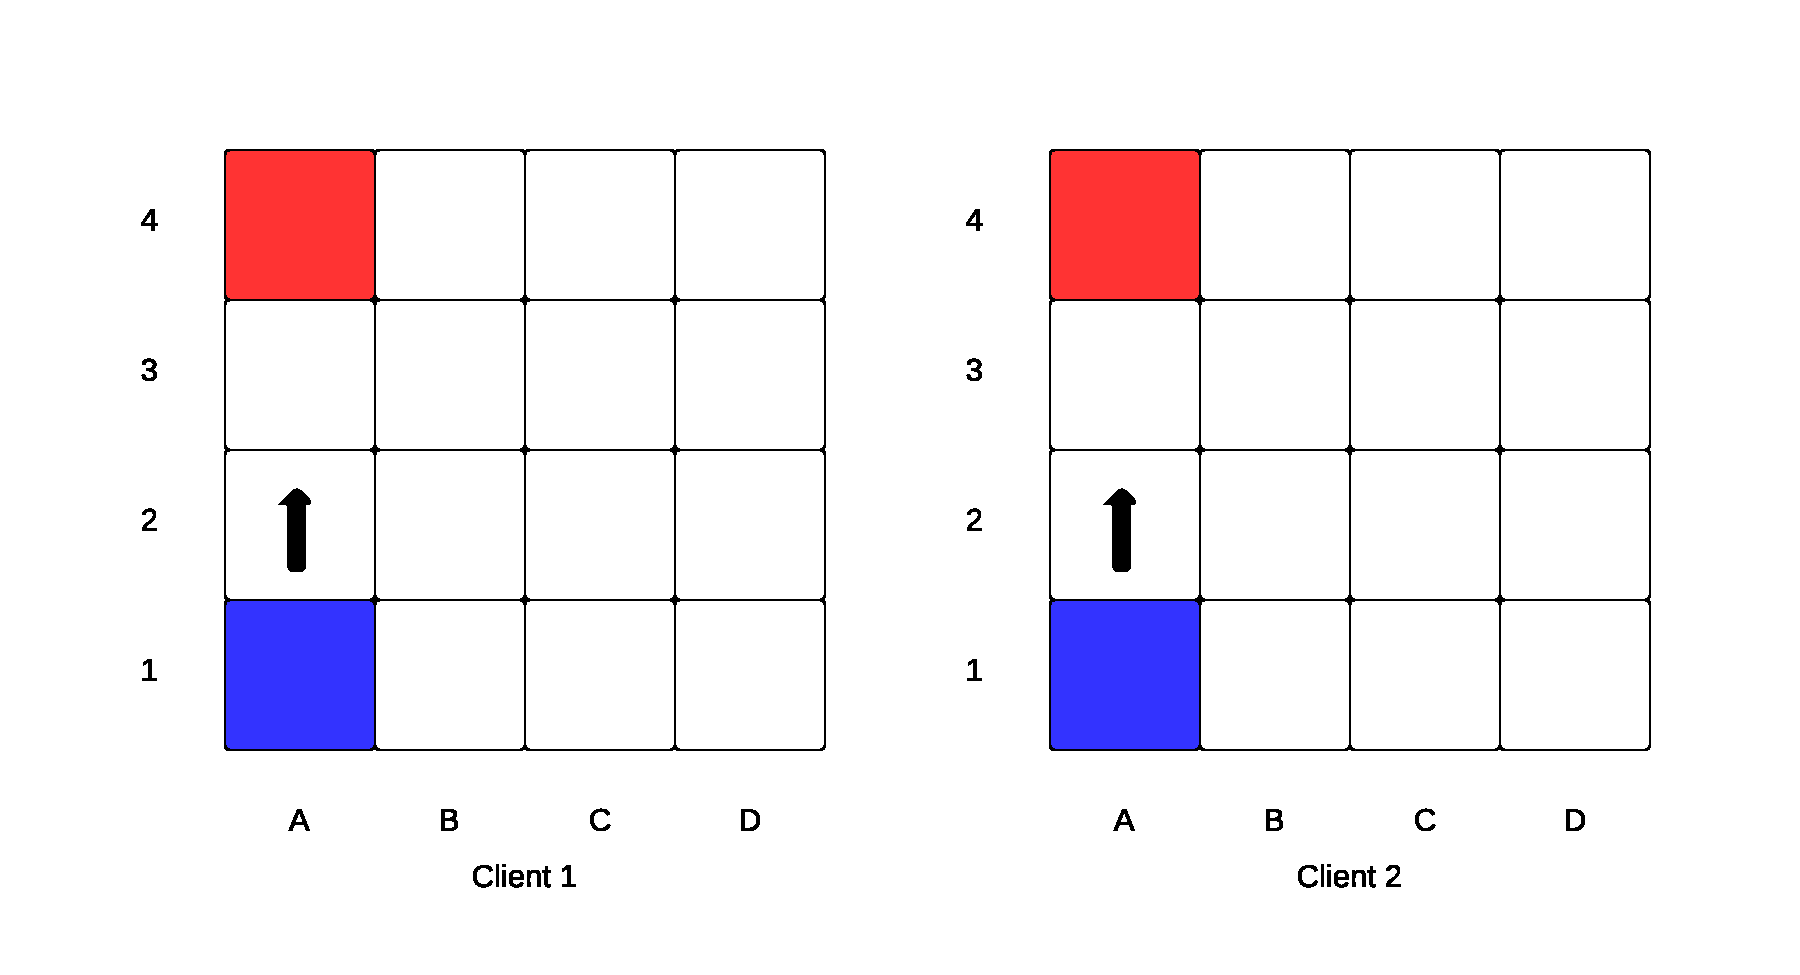
\includegraphics{res/computer_communication_architecture/ServerClientDesynchronisation1.pdf}
	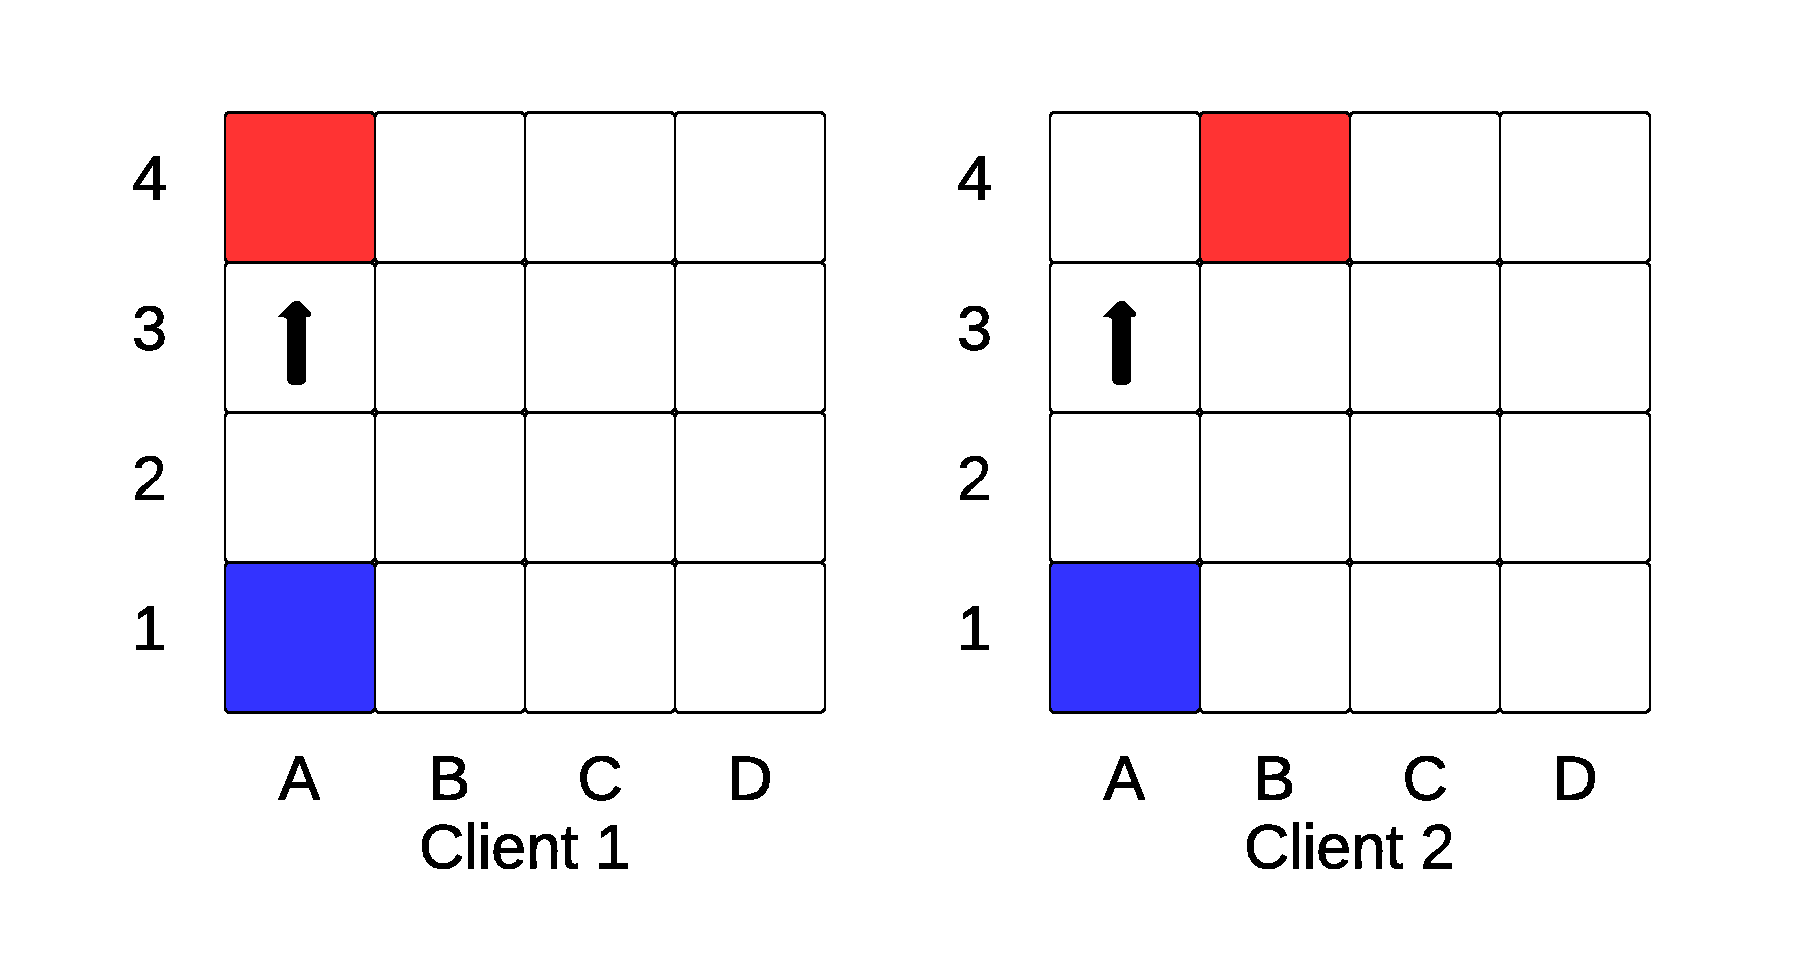
\includegraphics{res/computer_communication_architecture/ServerClientDesynchronisation2.pdf}
	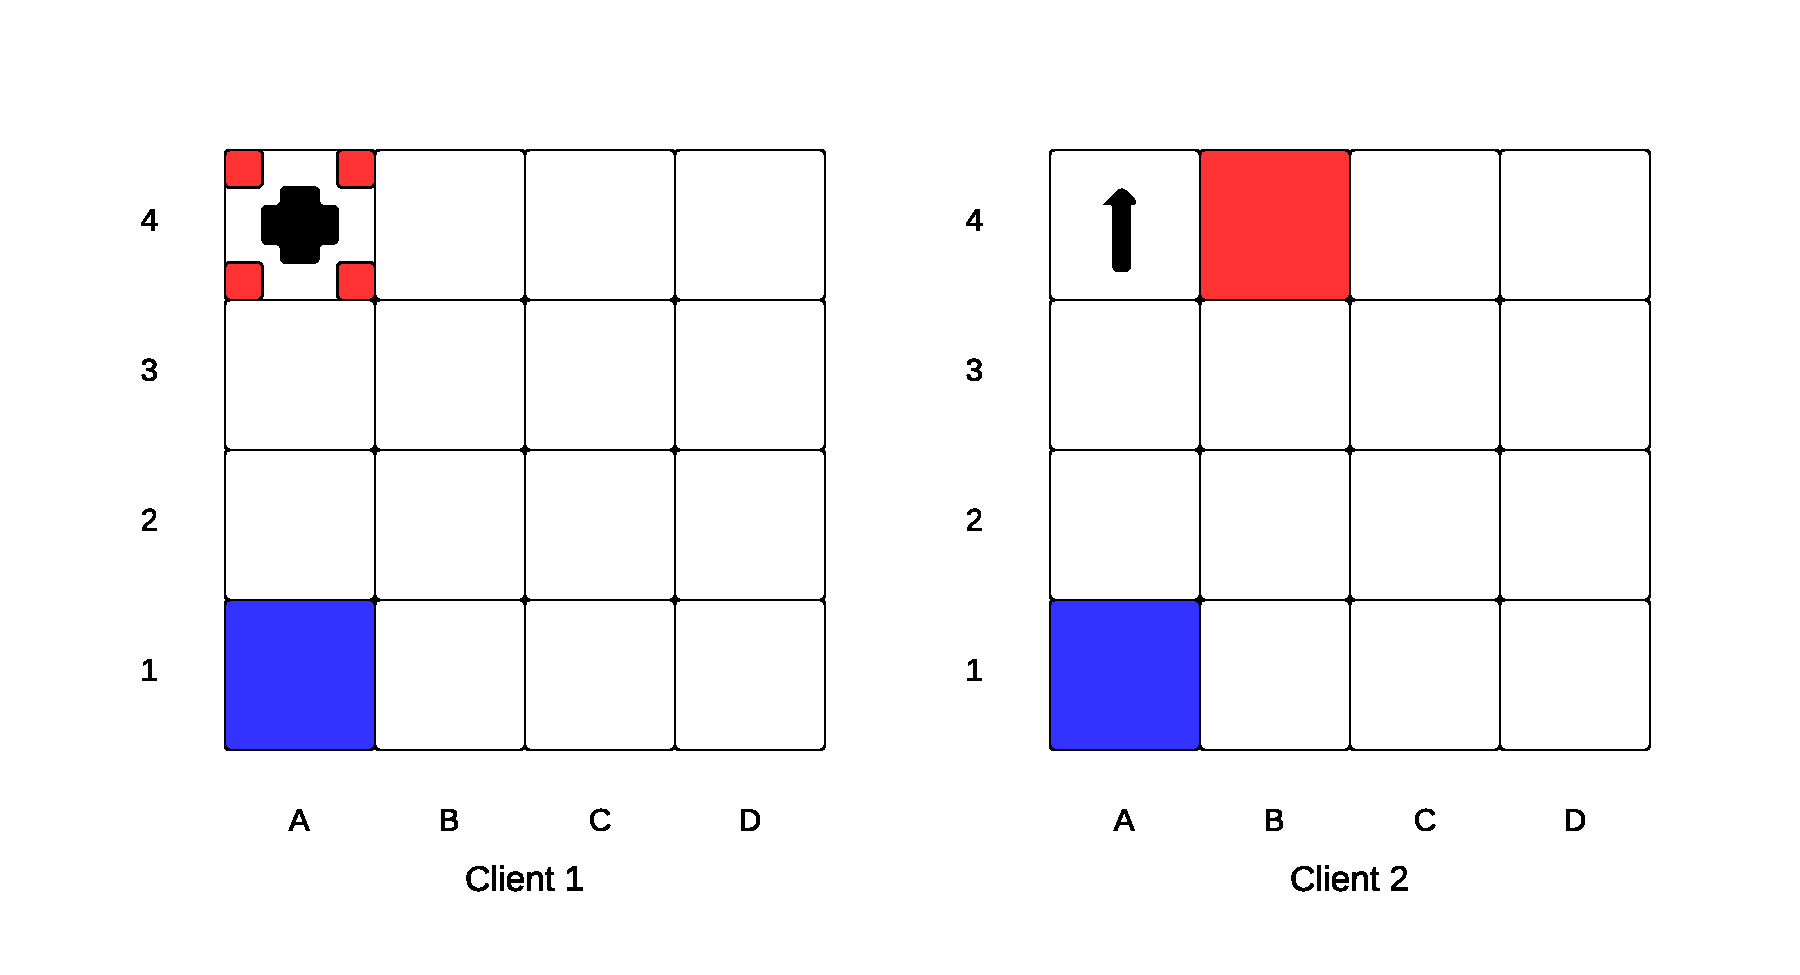
\includegraphics{res/computer_communication_architecture/ServerClientDesynchronisation3.pdf}		
	\caption[Desynchronisation when using lockstep]{Example of desynchronisation when using a lockstep strategy.}
	\label{fig:serverClientDesync}
\end{marginfigure}

In the simple server-client model the server and each of the clients have a copy of the game state, but instead of sharing the updates in a peer-to-peer fashion the server holds the master copy and it distributes canonical updates to the clients. When a player performs an action, the client sends a message to the server informing it of what happened. The server then applies the action to the game state to create an update which it sends to all of the clients. It must be ensured that all update messages are applied in the correct order, but this is much simpler to solve compared to the peer-to-peer version of the same problem since one machine is in charge of the decisions instead of a collective of machines.

The drawback to this approach is that clients must wait for the server to provide updates before they can show the new game state to the users. This can cause considerable lag when the network has high latency or is experiencing loss.

The final strategy was server-client with simulation. This is similar to simple server-client in that each node has a copy of the game state and the server's is deemed to be the master copy. However, clients also perform some simulation using client side prediction of the events about to occur in the very near future. If the client side prediction is incorrect then the authoratitive version of the game state held by the server will eventually correct the client's local state. This helps compensate for any latency on the network. The downside is that there can be noticeable changes in the game state if a correction is not received until a long time after the initial client side prediction failure occured. This strategy is popular with modern first person shooters such as \emph{Counter-Strike} and \emph{Team Fortress}.\cite{bernier2001simulation}

The simple server-client strategy was chosen for Project Serenity because of how much simpler it is to implement than the other two approaches. Also, since the game would be developed for LAN usage, latency would be less likely to be an issue. In the future, this strategy could also be extended to include some client side prediction and simulation.

One concern that was raised during these discussion was that of bandwidth. Would the volume of messages being passed between the clients and the server be too great? To answer this a basic design for the update messages was created and calculations were performed to estimate how large and numerous they would be. An example of a simple update message generated by the server would be to change the location of a ship in the world. Such a message would include: an identification number for the ship, new location coordinates, and new direction vector. The use of absolute values in this message instead of deltas reduces the chances of desynchronisation due to packet loss.

The original design of the messaging system only included three update messages:

\functions(addEntity, deleteEntity, updateEntity)
\begin{description}
	\item["addEntity"] Used to add a new entity to the game. It contains the entire details of the new entity.
	\item["deleteEntity"] Used to remove an existing entity from the game. It only needs to contain the entityID.
	\item["updateEntity"] The most common update. It is used to update existing entities. It contains an entire entity definition that is used to replace the existing one.
\end{description}

Having only three types of update was a very simple design and was easy to reason about. However, two of the three updates, "addEntity" and "updateEntity", contained entire entity objects which leads to large messages containing redundant information. Sending an entire entity definition across the network like this would be very slow and should only be done when absolutely necessary.

\begin{table}[t]
    \begin{tabular}{p{5em} p{15em} p{6em}}
    \toprule
    \emph{Update Type} & \emph{Description} & \emph{Fields} \\
    \midrule
    position & Used when both the ship's location and direction has changed & entityID, location, direction \\
    order & When a ship's order changes & entityID, order \\
    goal & When a ship's goal changes & entityID, goal \\
    plan & When a ship's plan changes & entityID, plan \\
    health & When a ship's hull or shields health changes & entityID, hull health, shield health \\ 
    \bottomrule
    \end{tabular}
    	\vspace{1em}
	\caption[Description of update messages]{Description of update messages.}
	\label{tab:updateMessageTypes}
\end{table}

The "addEntity" message does need to contain an entire entity since it is adding something new to the game. Since this message will primarily be used at the start of the game this is not a concern.

However, the "updateEntity" message is used extremely frequently since it would be sent every time an entity changes location, direction, is damaged, receives new orders, and so on. Evey time a single piece of data about the entity changes an entire entity is sent across the network. This would take up a large amount of bandwidth sending a great deal of information that has not actually changed. The solution to this problem was to split the "updateEntity" message into multiple different update types, one for each common usage of update. Table~\ref{tab:updateMessageTypes} shows the set of different update types that were devised.

With this change to the design, when an ship's field changes only that field is sent across the network. For example, if a ship's position is changed then only the position data is transmitted. This is significantly cheaper with regards to network usage compared to the monolithic "updateEntity".

\begin{margintable}
    \begin{tabular}{p{5em} p{5em}}
    \toprule
    \emph{Type} & \emph{Size (bytes)} \\
    \midrule
    \scalenote{"Int"} & 4 \\ 
    \scalenote{"Float"} & 4 \\
    \scalenote{"Double"} & 8 \\    
    \bottomrule
    \end{tabular}
    	\vspace{1em}
	\caption[Byte sizes of numeric fields]{Byte sizes of numeric fields.}
	\label{tab:typeSizes}
\end{margintable}

An analysis on the amount of traffic that would be sent using the new design was then undertaken to ensure that enough savings had been made. Some assumptions had to be made about the number of ships involved in a game, the number of game steps per second, and so on, but in these cases a worst case scenario was assumed to make sure nothing was underestimated. To perform the analysis, the size of each update message and their frequency needed to be estimated.

\begin{margintable}
    \begin{tabular}{p{5em} p{5em} p{5em}}
    \toprule
    \emph{Field Name} & \emph{Size (bytes)} \\
    \midrule
    entityID & 4 \\ 
    location & 8 \\
    direction & 8 \\ 
    order & 15 \\
    goal & 9 \\ 
    plan & 100 \\ 
    hull & 4  \\ 
    shield & 4  \\  
    \bottomrule
    \end{tabular}
    	\vspace{1em}
    	%todo somebody verify caption please!
	\caption[Byte sizes of update fields]{Byte sizes of update fields.}
	\label{tab:fieldSizes}
\end{margintable}

First, the sizes of various common data types, such as "Int" and "Float", were collated. These figures are shown in Table~\ref{tab:typeSizes}. With these figures available it was possible to determine the sizes of different fields in the update messages by working out the type of each field. This data is shown in Table~\ref{tab:fieldSizes}. For example, a location is known to be a pair of "Float"s and so it can be assumed to consume eight bytes.

Secondly, the size of individual fields was used to calculate the size of whole messages which include multiple fields. Then the frequency at which different messages would be sent by the server was estimated. This data is shown in Table~\ref{tab:updateMessageStats}.

\begin{margintable}
    \begin{tabular}{p{5em} p{5em} p{5em}}
    \toprule
    \emph{Update Type} & \emph{Size (bytes)} & \emph{Frequency} \\
    \midrule
    position & 20 & 1 \\ 
    order & 19 & 0.2 \\
    goal & 14 & 0.3 \\
    plan & 104 & 0.3 \\
    health & 12 & 0.1 \\   
    \bottomrule
    \end{tabular}
    	\vspace{1em}
	\caption[Size and frequency of update messages]{Size of each update message and its average frequency per game step.}
	\label{tab:updateMessageStats}
\end{margintable}

The number of bytes sent to a single client in a single game step was calculated from the data in Table~\ref{tab:updateMessageStats}:

\begin{align*}
bytes &= 20 \times 1 + 19 \times 0.2 + 14 \times 0.3 + 104 \times 0.3 + 12 \times 0.1 \\
      &= 60.4
\end{align*}

Let $S$ be the number of game steps per second, and $N$ be the number of clients connected to the server. Then the number of bytes the server sends per second is $S \times N \times 60.4$. This formula to calculate network traffic per second was then applied to various likely values of $S$ and $N$. The results are shown in Table~\ref{tab:networkRequirements}.

\begin{margintable}
    \begin{tabular}{p{5em} p{5em} p{5em}}
    \toprule
    \emph{Steps Per Second} & \emph{Number of Clients} & \emph{kB/s} \\
    \midrule
    15 & 2 & 1.77 \\
    15 & 4 & 3.54 \\
    15 & 8 & 7.08 \\
    15 & 16 & 14.16 \\
    30 & 2 & 3.54 \\
    30 & 4 & 7.08 \\
    30 & 8 & 14.16 \\
    30 & 16 & 28.31 \\
    45 & 2 & 5.31 \\
    45 & 4 & 10.62 \\
    45 & 8 & 21.23 \\
    45 & 16 & 42.47 \\
    60 & 2 & 7.08 \\
    60 & 4 & 14.16 \\
    60 & 8 & 28.31 \\
    60 & 16 & 56.62 \\
    \bottomrule
    \end{tabular}
    	\vspace{1em}
	\caption[Estimation of network requirements]{
	Estimate of traffic generated for various game setups.}
	\label{tab:networkRequirements}
\end{margintable}

For the greatest expected values of $S$ and $N$, 60 and 16 respectively, the network usage per second is only 56.62 kilobytes. This is easily acceptable for a multiplayer game running on a LAN.
